\documentclass[12pt]{article}
\usepackage[utf8]{inputenc}
\usepackage{graphicx}
\graphicspath{ {images/} }
\usepackage[citestyle=ieee]{biblatex}
\addbibresource{refrences.bib}

\usepackage{listings}
\usepackage{color}

\definecolor{dkgreen}{rgb}{0,0.6,0}
\definecolor{gray}{rgb}{0.5,0.5,0.5}
\definecolor{mauve}{rgb}{0.58,0,0.82}

\lstset{frame=tb,
  language=Java,
  aboveskip=3mm,
  belowskip=3mm,
  showstringspaces=false,
  columns=flexible,
  basicstyle={\small\ttfamily},
  numbers=none,
  numberstyle=\tiny\color{gray},
  keywordstyle=\color{blue},
  commentstyle=\color{dkgreen},
  stringstyle=\color{mauve},
  breaklines=true,
  breakatwhitespace=true,
  tabsize=3
}



\title{Data Structure Research Paper \\
    \large BQ: A Lock-Free Queue with Batching
}
\author{John Mirschel and Timothy Rigby}
\date{March 2019}

\begin{document}

\maketitle


\begin{abstract}
This paper describes an implementation of a lock-free queue that utilizes batching to increase performance by up to 16x over standard lock-free queues. We attempted to implement the design and algorithms from the original research paper BQ: A Lock-Free Queue with Batching  and tried to reproduce similar functionality and performance. The original implementation of this data structure was done in C++, but we wanted to try and build this in Java so we could compare the results of how the data structure performs in two different languages. 
\end{abstract}


\section{Introduction}
Our implementation of the lock-free queue provides all of the functionality available to a sequential queue. Our lock free batching extension builds upon the simple concurrent lock free queue implemented by Michael and Scott by vastly improving on scalability of the concurrent lock free queue. A concurrent queue has two access points of high contention, the head of the queue from which nodes are dequeued and the tail of the queue into where new nodes are enqueued. This inherently limits throughput of the data structure as only one thread can enqueue and one thread can dequeue at a time. Our version of a lock-free queue uses the idea of the future programming construct to perform batching operations as first seen in the paper written by Kogan and Herlithy\parencite{r4}. Batching means to just group a sequence of standard operations to just one single batch operation, which then applies them together to the shared data structure. 

Kogan and Herlithy originally proposed that operations with the same type (enqueue or dequeue) get added to the shared queue all at once. This means they execute each subsequence of enqueues together by appending them in order to the tail of the queue, and each subsequence of dequeues is removed from the head of the list all at the same time. The problem with this implementation is that performance can degrade if the operations in the batch frequently switch between enqueue and dequeue, as their implementation only allows for a batch to be built from sequential and like operations. The algorithm we implemented improves on this idea by batching these operations locally. Local batching allows our algorithm to handle both enqueue and dequeue operations in any order and build the result before applying it to the shared queue. This means it applies the batch operation all at once to the shared queue to reduce contention between multiple threads. This helps solve the problem that concurrent queues have with the contention of the head and tail pointers by batching these operations locally, which reduces the number of access attempts to the shared queue and improves scalability. 


\section{Related Works}
Lorem ipsum dolor sit amet, ne vix omnes philosophia, nostrud detracto imperdiet an cum. Pro fuisset appetere eu, stet facer nominavi te vix. Ut eam postea molestie. Accusata pertinacia ut sed, id nec esse scripta invenire, nibh rebum dicunt vim ei. Ridens aliquid vel eu, id duo putent repudiandae, id nihil audire euismod vix. Alii mazim facilisi pro id.

Vel ad dictas delicata deterruisset. Dolorem contentiones no vix, saperet nominavi senserit nec ne. Simul timeam sadipscing per ei, id summo patrioque his. Pri labitur dissentiunt at.

Ne vim tibique laboramus. Sit denique sapientem incorrupte in. Pri ex inciderint voluptatibus, eum id albucius elaboraret ullamcorper. Ex dicit minimum conceptam his.

Eu diam case tincidunt vel, facilis scribentur ad vis, affert minimum intellegat eum te. Falli virtute duo in, ad ius aliquip albucius. Ex eam quando oblique. Cu cum legendos antiopam. Ut paulo aperiri tamquam his, vel an vide eirmod.

Omnium aliquam tacimates duo ea, meis scripta expetenda nec ad, mel fugit discere ne. Vim et quodsi impetus efficiendi. Quo appetere inimicus ei. Id eum saperet ornatus. Ad oblique vituperata reformidans has. Ex odio animal deleniti vel, dicta adipisci disputationi ea has, ad mandamus electram sadipscing mel.

\section{Overview}
Lorem ipsum dolor sit amet, eam an simul delicatissimi, sed bonorum inermis at. Postea postulant adversarium ad per, cu qui eirmod recusabo tincidunt, idque harum temporibus at has. Esse omnes conceptam ei quo. Alia viderer vel at, cu vim nulla antiopam constituto, mel in propriae inimicus. Reque dicam laboramus has cu.\parencite{r1}

Ignota neglegentur his ex. An putent essent mediocritatem sea, pri vitae soluta albucius eu. Ea mazim lobortis pri, putent dissentias has in, duo ut mucius audire. Ea his illud salutatus, te dolor conceptam liberavisse usu.
\begin{figure}[ht]
\centering
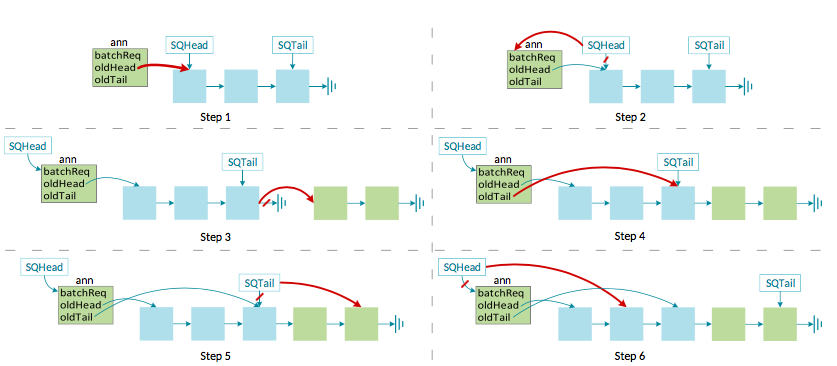
\includegraphics[scale=0.35]{img1}
\caption{An example image}
\label{fig: test_img}
\end{figure}

Exerci explicari at nec, ut vix ceteros denique. Ad vis erat utinam. Duis vocent lucilius eos id, an usu lorem melius scripta. Quodsi platonem in mea, iudico nominavi ea vim. Dicant vidisse inciderint no qui, ius cu reque tempor nostrum. Putent iisque no sed, quis vide ad eum.

\section{Algorithm Details}

\setcounter{subsection}{0}
The Batching Queue extension to the Lock Free Queue allows for deferred operations to operate in batches of operations rather than having each enqueue and dequeue execute on the shared queue as they are called. The deferring of these operations allows for the user to aggregate pending operations within each thread to be executed at a later time. When a future method is called, either enqueue or dequeue, a Future object is returned to the caller, who may evaluate it later. The execution of operations on the shared queue is delayed until the user explicitly evaluates the future of a deferred operation or a standard queue operation is called. At the point of evaluation, the pending operations of a thread are gathered to a single batched operation to be applied to the shared queue. After which the batch execution is finalized by locally filling in the return values of the pending operations. This locally batched execution and value filling reduces the overhead of having multiple threads compete for alteration of the shared queue.\newline





\subsection{Data Structures}
\begin{lstlisting} 
public class Node<T>    {T val; AtomicReference<Node<T>> next;}

public class Future<T> {T returnVal; boolean isDone;}

public class NodeWithCount<T> {Node<T> node; int count;}

public class FutureOp<T> {boolean isEnqueue; Future<T> future;}

public class NodeCountOrAnn {
    boolean isAnnouncement;
    NodeWithCount nodeWCount;
    Announcement announcement;
}


public class BatchRequest<T>{
    Node<T> firstEnq;
    Node<T> lastEnq;
    int numEnqs;
    int numDeqs;
    int numExcessDeqs;
}

public class NodeCountOrAnn {
    boolean isAnnouncement;
    NodeWithCount nodeWCount;
    Announcement announcement;
}

public class ThreadData<T> {
    Queue<FutureOp> opsQueue;
    Node<T> enqHead;
    Node<T> enqTail;
    int numEnqs;
    int numDeqs;
    int numExcessDeqs;
}\end{lstlisting}

\begin{enumerate}
 \item \textbf{Node Class: } The Node class is just a standard node class for a linked list implementation.
  \item \textbf{Future Class: }The Future class is going to be containing a \textit{result} which will be holding the return value of the deferred operation that generated the Future, and a isDone value so we now if the deferred operation has been completed.
  \item \textbf{NodeWithCount Class: } The NodeWithCount class is a standard node class but with a integer counter attached to perform double CAS operations.
  \item \textbf{FutureOp Class: }The FutureOp class is used to hold a deferred operation such as an enqueue or a dequeue. It will also hold a copy of a Future to be used for evaluation.
  \item \textbf{BatchRequest Class: } The BatchRequest class will be prepared by a thread that needs to initiate a batch, and it will hold the details of the batches operations. The fields \textit{firstEnq} and \textit{lastEnq} are references to the first and last nodes of the pending items to be put in to the shared queue. While the fields  \textit{numEnqs}, \textit{numDeqs}, and \textit{numExcessDeqs} are details about the batch.
  \item \textbf{NodeCountOrAnn Class: }The NodeCountOrAnn is used to hold either an Annoouncement or a NodeWithCount. The class will have a boolean value \textit{isAnnouncement} if this is set to true, then we are using the \textit{announcement}field, and if it false then we are using the \textit{nodeWCount} field. 
  \item \textbf{ThreadData Class: } This is the class that will be used to store all the local data for a given thread. The \textit{opsQueue} is just a standard non thread-safe Queue of FutureOps that is used to store all operations received by a thread. The \textit{enqHead} and \textit{enqTail} fields are used to access and keep track of the queue of FutureOps. The last three fields \textit{numEnqs}, \textit{numDeqs}, and \textit{numExcessDeqs}are used to store the prepossessing data so we are able to manage where the head and tail should be pointing after applying a batch. 
\end{enumerate}
\newpage


\subsection{Algorithm Implementation}
The following methods are used internally to apply operations to the shared queue: \textit{EnqueueToShared}, \textit{DequeueFromShared} and \textit{ExecuteBatch}. To help a concurrent batch execution and obtain the new head, they call the \textit{HelpAnnAndGetHead} auxiliary method. To carry out a batch, the \textit{ExecuteAnn} auxiliary method is called. It’s caller can be either the batch’s initiating thread or a helping thread that encountered the announcement while trying to complete its own operation.\newline

\textbf{EnqueueToShared: } This method appends an item after the tail of the shared queue using two CAS operations. It first updates the shared tail’s next node to point to the new node and item, and then updates the shared tail to point to the new node and item. If another thread obstructs operation by enqueueing its own item concurrently, \textit{EnqueueToShared} will try and help complete the obstructing operation before retrying its own operation. This is possible through the use of two CAS operations to link the node and update the shared tail. This method can be obstructed by either a singular operation or a batch operation.\newline

\textbf{DequeueFromShare: } If the queue is not empty when the dequeue operation takes effect, this method extracts an item from the head of the shared queue and returns it. Otherwise, it returns NULL if taking effect on an empty queue. This method will also help assist ongoing batch operations to complete first through its calling of \textit{HelpAnnAndGetHead} in its execution.\newline

\textbf{HelpAnnAndGetHead: } This auxiliary method helps announcements to complete their execution by returning the head \textit{NodeWithCount} if there is no announcement in place or the Announcement object if there is an announcement in progress, allowing the calling thread to assist execution. This method will return the head of the shared queue, which is a \textit{NodeCountOrAnnouncement} object.\newline

\textbf{ExecuteBatch: } This method is responsible for executing the batch. It receives a \textit{BatchRequest} object and creates a new announcement for it. Before storing this announcement in the head it checks to see if the head contains an announcement. If the head already contains an announcement, it helps it to complete its execution. Otherwise, this method will replace the head of the shared queue with this new announcement object, encouraging all other threads to help it complete.\newline

\textbf{ExecuteAnnouncement: } is called by \textit{ExecuteBatch} after installing an Announcement object in the shared head or by other threads that otherwise encounter an Announcement object in the shared head. \textit{ExecuteAnnouncement} will carry out an Announcement’s batch. If any of the steps in the execution of the batch have been completed by a competing thread, the method moves on to the next step without taking effect on the shared queue.\newline

The first step of \textit{ExecuteAnnouncement} is to make sure that the items in the Announcement is linked to the shared queue, and that the old tail to which they were appended has been recorded in the Announcement object. If the items have already been appended to the queue and the old tail has been recorded in the Announcement it is clear that another thread has completed the linking, and the method breaks out of the linkage loop. Otherwise, we try to link the items to the queue though a compare and set operation on the next pointer of the current tail node of the shared queue. We then check whether the compare and set operated succeeded in linking the items. If the items were successfully linked, the old tail reference is stored to signify the successful linkage. Otherwise, we would try and help any other obstructing operations and restart the attempt at the linkage\newline

The next step in the method is to update the reference of the shared queue’s tail to reflect the newly appended nodes. The last step is to call updateHead so we can update the head of the shared queue to point to the last node that was dequeued by the batch. By doing so, this will also uninstall the announcement that was inserted in to the shared queues head and it will complete its handling.\newline

\textbf{UpdateHead: } This methods main purpose is to update the head to the correct location after a batch operation is complete. The algorithm for this process is as follows: If the number of the batch's successful dequeues is at least the size of of the queue before applying the batch, then the head is determined by over \textit{uccess f ulDeqsNum} - \textit{oldQueueSize} nodes, starting at the position of the node pointed to by old tail. Otherwise, we determine it by passing over \textit{successfulDeqsNum} and by starting at the old dummy node. Finally, the head is moved to the correct position after the batch is applied. 

\textbf{Interface Methods: } The following methods are ones that are exposed to the user. They consist of \textit{Enqueue}, \textit{Dequeue}, \textit{FutureEnqueue}, \textit{FutureDequeue} and \textit{Evaluate}. The first method \textit{Enqueue}, is for if the user is just trying to insert a single item in to the shared queue. By calling \textit{Enqueue} the thread will just push one single item on to the shared queue. \textit{Dequeue} works similar to the \textit{Enqueue} method in that it will just attempt to dequeue one item from the shared queue. If the queue is empty then \textit{Dequeue} will just return null. \textit{FutureEnqueue} is for the user to create a \textit{FutureOp} object representing an enqueue operation to be inserted in to the \textit{ThreadData} opsQueue. \textit{FutureEnqueue} will also keep track of the number of pending enqueue operations so it knows the amount of enqueues in the batch. \textit{FutureDequeue} operates in a similar way as \textit{FutureEnqueue}, but is instead handling dequeue operations and keeping track of the number of pending dequeues. The final method is \textit{Evaluate}, which receives a \textit{Future} and makes sure that it is applied when the method returns. If the Future has already been applied from the outset, then the result is immediately returned. Otherwise, all the items in the local \textit{ThreadData} queue \textit{opsQueue} will be applied all at once by calling the method \textit{ExecuteBatch}.



\newpage

\printbibliography
\end{document}
